\documentclass[1p]{elsarticle_modified}
%\bibliographystyle{elsarticle-num}

%\usepackage[colorlinks]{hyperref}
%\usepackage{abbrmath_seonhwa} %\Abb, \Ascr, \Acal ,\Abf, \Afrak
\usepackage{amsfonts}
\usepackage{amssymb}
\usepackage{amsmath}
\usepackage{amsthm}
\usepackage{scalefnt}
\usepackage{amsbsy}
\usepackage{kotex}
\usepackage{caption}
\usepackage{subfig}
\usepackage{color}
\usepackage{graphicx}
\usepackage{xcolor} %% white, black, red, green, blue, cyan, magenta, yellow
\usepackage{float}
\usepackage{setspace}
\usepackage{hyperref}

\usepackage{tikz}
\usetikzlibrary{arrows}

\usepackage{multirow}
\usepackage{array} % fixed length table
\usepackage{hhline}

%%%%%%%%%%%%%%%%%%%%%
\makeatletter
\renewcommand*\env@matrix[1][\arraystretch]{%
	\edef\arraystretch{#1}%
	\hskip -\arraycolsep
	\let\@ifnextchar\new@ifnextchar
	\array{*\c@MaxMatrixCols c}}
\makeatother %https://tex.stackexchange.com/questions/14071/how-can-i-increase-the-line-spacing-in-a-matrix
%%%%%%%%%%%%%%%

\usepackage[normalem]{ulem}

\newcommand{\msout}[1]{\ifmmode\text{\sout{\ensuremath{#1}}}\else\sout{#1}\fi}
%SOURCE: \msout is \stkout macro in https://tex.stackexchange.com/questions/20609/strikeout-in-math-mode

\newcommand{\cancel}[1]{
	\ifmmode
	{\color{red}\msout{#1}}
	\else
	{\color{red}\sout{#1}}
	\fi
}

\newcommand{\add}[1]{
	{\color{blue}\uwave{#1}}
}

\newcommand{\replace}[2]{
	\ifmmode
	{\color{red}\msout{#1}}{\color{blue}\uwave{#2}}
	\else
	{\color{red}\sout{#1}}{\color{blue}\uwave{#2}}
	\fi
}

\newcommand{\Sol}{\mathcal{S}} %segment
\newcommand{\D}{D} %diagram
\newcommand{\A}{\mathcal{A}} %arc


%%%%%%%%%%%%%%%%%%%%%%%%%%%%%5 test

\def\sl{\operatorname{\textup{SL}}(2,\Cbb)}
\def\psl{\operatorname{\textup{PSL}}(2,\Cbb)}
\def\quan{\mkern 1mu \triangleright \mkern 1mu}

\theoremstyle{definition}
\newtheorem{thm}{Theorem}[section]
\newtheorem{prop}[thm]{Proposition}
\newtheorem{lem}[thm]{Lemma}
\newtheorem{ques}[thm]{Question}
\newtheorem{cor}[thm]{Corollary}
\newtheorem{defn}[thm]{Definition}
\newtheorem{exam}[thm]{Example}
\newtheorem{rmk}[thm]{Remark}
\newtheorem{alg}[thm]{Algorithm}

\newcommand{\I}{\sqrt{-1}}
\begin{document}

%\begin{frontmatter}
%
%\title{Boundary parabolic representations of knots up to 8 crossings}
%
%%% Group authors per affiliation:
%\author{Yunhi Cho} 
%\address{Department of Mathematics, University of Seoul, Seoul, Korea}
%\ead{yhcho@uos.ac.kr}
%
%
%\author{Seonhwa Kim} %\fnref{s_kim}}
%\address{Center for Geometry and Physics, Institute for Basic Science, Pohang, 37673, Korea}
%\ead{ryeona17@ibs.re.kr}
%
%\author{Hyuk Kim}
%\address{Department of Mathematical Sciences, Seoul National University, Seoul 08826, Korea}
%\ead{hyukkim@snu.ac.kr}
%
%\author{Seokbeom Yoon}
%\address{Department of Mathematical Sciences, Seoul National University, Seoul, 08826,  Korea}
%\ead{sbyoon15@snu.ac.kr}
%
%\begin{abstract}
%We find all boundary parabolic representation of knots up to 8 crossings.
%
%\end{abstract}
%\begin{keyword}
%    \MSC[2010] 57M25 
%\end{keyword}
%
%\end{frontmatter}

%\linenumbers
%\tableofcontents
%
\newcommand\colored[1]{\textcolor{white}{\rule[-0.35ex]{0.8em}{1.4ex}}\kern-0.8em\color{red} #1}%
%\newcommand\colored[1]{\textcolor{white}{ #1}\kern-2.17ex	\textcolor{white}{ #1}\kern-1.81ex	\textcolor{white}{ #1}\kern-2.15ex\color{red}#1	}

{\Large $\underline{11a_{217}~(K11a_{217})}$}

\setlength{\tabcolsep}{10pt}
\renewcommand{\arraystretch}{1.6}
\vspace{1cm}\begin{tabular}{m{100pt}>{\centering\arraybackslash}m{274pt}}
\multirow{5}{120pt}{
	\centering
	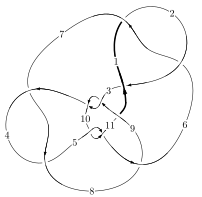
\includegraphics[width=112pt]{../../../GIT/diagram.site/Diagrams/png/466_11a_217.png}\\
\ \ \ A knot diagram\footnotemark}&
\allowdisplaybreaks
\textbf{Linearized knot diagam} \\
\cline{2-2}
 &
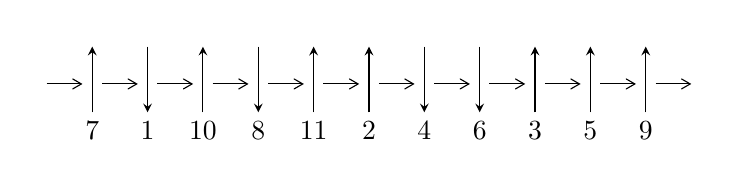
\begin{tikzpicture}[x=20pt, y=17pt]
	% nodes
	\node (C0) at (0, 0) {};
	\node (C1) at (1, 0) {};
	\node (C1U) at (1, +1) {};
	\node (C1D) at (1, -1) {7};

	\node (C2) at (2, 0) {};
	\node (C2U) at (2, +1) {};
	\node (C2D) at (2, -1) {1};

	\node (C3) at (3, 0) {};
	\node (C3U) at (3, +1) {};
	\node (C3D) at (3, -1) {10};

	\node (C4) at (4, 0) {};
	\node (C4U) at (4, +1) {};
	\node (C4D) at (4, -1) {8};

	\node (C5) at (5, 0) {};
	\node (C5U) at (5, +1) {};
	\node (C5D) at (5, -1) {11};

	\node (C6) at (6, 0) {};
	\node (C6U) at (6, +1) {};
	\node (C6D) at (6, -1) {2};

	\node (C7) at (7, 0) {};
	\node (C7U) at (7, +1) {};
	\node (C7D) at (7, -1) {4};

	\node (C8) at (8, 0) {};
	\node (C8U) at (8, +1) {};
	\node (C8D) at (8, -1) {6};

	\node (C9) at (9, 0) {};
	\node (C9U) at (9, +1) {};
	\node (C9D) at (9, -1) {3};

	\node (C10) at (10, 0) {};
	\node (C10U) at (10, +1) {};
	\node (C10D) at (10, -1) {5};

	\node (C11) at (11, 0) {};
	\node (C11U) at (11, +1) {};
	\node (C11D) at (11, -1) {9};
	\node (C12) at (12, 0) {};

	% arrows
	\draw[->,>={angle 60}]
	(C0) edge (C1) (C1) edge (C2) (C2) edge (C3) (C3) edge (C4) (C4) edge (C5) (C5) edge (C6) (C6) edge (C7) (C7) edge (C8) (C8) edge (C9) (C9) edge (C10) (C10) edge (C11) (C11) edge (C12) ;	\draw[->,>=stealth]
	(C1D) edge (C1U) (C2U) edge (C2D) (C3D) edge (C3U) (C4U) edge (C4D) (C5D) edge (C5U) (C6D) edge (C6U) (C7U) edge (C7D) (C8U) edge (C8D) (C9D) edge (C9U) (C10D) edge (C10U) (C11D) edge (C11U) ;
	\end{tikzpicture} \\
\hhline{~~} \\& 
\textbf{Solving Sequence} \\ \cline{2-2} 
 &
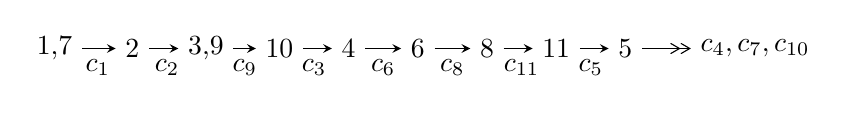
\begin{tikzpicture}[x=25pt, y=7pt]
	% node
	\node (A0) at (-1/8, 0) {1,7};
	\node (A1) at (1, 0) {2};
	\node (A2) at (33/16, 0) {3,9};
	\node (A3) at (25/8, 0) {10};
	\node (A4) at (33/8, 0) {4};
	\node (A5) at (41/8, 0) {6};
	\node (A6) at (49/8, 0) {8};
	\node (A7) at (57/8, 0) {11};
	\node (A8) at (65/8, 0) {5};
	\node (C1) at (1/2, -1) {$c_{1}$};
	\node (C2) at (3/2, -1) {$c_{2}$};
	\node (C3) at (21/8, -1) {$c_{9}$};
	\node (C4) at (29/8, -1) {$c_{3}$};
	\node (C5) at (37/8, -1) {$c_{6}$};
	\node (C6) at (45/8, -1) {$c_{8}$};
	\node (C7) at (53/8, -1) {$c_{11}$};
	\node (C8) at (61/8, -1) {$c_{5}$};
	\node (A9) at (10, 0) {$c_{4},c_{7},c_{10}$};

	% edge
	\draw[->,>=stealth]	
	(A0) edge (A1) (A1) edge (A2) (A2) edge (A3) (A3) edge (A4) (A4) edge (A5) (A5) edge (A6) (A6) edge (A7) (A7) edge (A8) ;
	\draw[->>,>={angle 60}]	
	(A8) edge (A9);
\end{tikzpicture} \\ 

\end{tabular} \\

\footnotetext{
The image of knot diagram is generated by the software ``\textbf{Draw programme}" developed by Andrew Bartholomew(\url{http://www.layer8.co.uk/maths/draw/index.htm\#Running-draw}), where we modified some parts for our purpose(\url{https://github.com/CATsTAILs/LinksPainter}).
}\phantom \\ \newline 
\centering \textbf{Ideals for irreducible components\footnotemark of $X_{\text{par}}$} 
 
\begin{align*}
I^u_{1}&=\langle 
1.17366\times10^{130} u^{87}-2.47035\times10^{130} u^{86}+\cdots+1.30550\times10^{131} b+1.73562\times10^{131},\\
\phantom{I^u_{1}}&\phantom{= \langle  }-1.20844\times10^{131} u^{87}-1.95249\times10^{131} u^{86}+\cdots+3.91650\times10^{131} a+2.77458\times10^{132},\\
\phantom{I^u_{1}}&\phantom{= \langle  }u^{88}+u^{87}+\cdots-15 u-9\rangle \\
I^u_{2}&=\langle 
- u^{18}+u^{17}+\cdots+b-1,\;2 u^{18}-3 u^{17}+\cdots+a+7,\;u^{19}+6 u^{17}+\cdots+2 u-1\rangle \\
\\
\end{align*}
\raggedright * 2 irreducible components of $\dim_{\mathbb{C}}=0$, with total 107 representations.\\
\footnotetext{All coefficients of polynomials are rational numbers. But the coefficients are sometimes approximated in decimal forms when there is not enough margin.}
\newpage
\renewcommand{\arraystretch}{1}
\centering \section*{I. $I^u_{1}= \langle 1.17\times10^{130} u^{87}-2.47\times10^{130} u^{86}+\cdots+1.31\times10^{131} b+1.74\times10^{131},\;-1.21\times10^{131} u^{87}-1.95\times10^{131} u^{86}+\cdots+3.92\times10^{131} a+2.77\times10^{132},\;u^{88}+u^{87}+\cdots-15 u-9 \rangle$}
\flushleft \textbf{(i) Arc colorings}\\
\begin{tabular}{m{7pt} m{180pt} m{7pt} m{180pt} }
\flushright $a_{1}=$&$\begin{pmatrix}1\\0\end{pmatrix}$ \\
\flushright $a_{7}=$&$\begin{pmatrix}0\\u\end{pmatrix}$ \\
\flushright $a_{2}=$&$\begin{pmatrix}1\\- u^2\end{pmatrix}$ \\
\flushright $a_{3}=$&$\begin{pmatrix}u^2+1\\- u^2\end{pmatrix}$ \\
\flushright $a_{9}=$&$\begin{pmatrix}0.308550 u^{87}+0.498528 u^{86}+\cdots+7.54550 u-7.08434\\-0.0899012 u^{87}+0.189226 u^{86}+\cdots-2.55127 u-1.32947\end{pmatrix}$ \\
\flushright $a_{10}=$&$\begin{pmatrix}-0.386032 u^{87}-0.283155 u^{86}+\cdots+12.0176 u-0.729770\\-0.256563 u^{87}+0.494342 u^{86}+\cdots-0.570209 u-4.79156\end{pmatrix}$ \\
\flushright $a_{4}=$&$\begin{pmatrix}0.317057 u^{87}-0.164745 u^{86}+\cdots-15.3332 u+2.84818\\-0.127635 u^{87}+0.423062 u^{86}+\cdots+4.82042 u-0.610035\end{pmatrix}$ \\
\flushright $a_{6}=$&$\begin{pmatrix}- u\\u^3+u\end{pmatrix}$ \\
\flushright $a_{8}=$&$\begin{pmatrix}-0.244942 u^{87}-0.153358 u^{86}+\cdots+12.6279 u-2.44254\\-0.265588 u^{87}+0.498825 u^{86}+\cdots-1.17630 u-5.08573\end{pmatrix}$ \\
\flushright $a_{11}=$&$\begin{pmatrix}-0.728320 u^{87}-0.445892 u^{86}+\cdots+23.4775 u+5.97101\\0.299986 u^{87}+0.213630 u^{86}+\cdots-6.17882 u-4.63479\end{pmatrix}$ \\
\flushright $a_{5}=$&$\begin{pmatrix}-0.566401 u^{87}+0.182126 u^{86}+\cdots+13.2863 u+1.44734\\0.921798 u^{87}+0.106995 u^{86}+\cdots-9.79027 u-4.16570\end{pmatrix}$\\ \flushright $a_{5}=$&$\begin{pmatrix}-0.566401 u^{87}+0.182126 u^{86}+\cdots+13.2863 u+1.44734\\0.921798 u^{87}+0.106995 u^{86}+\cdots-9.79027 u-4.16570\end{pmatrix}$\\&\end{tabular}
\flushleft \textbf{(ii) Obstruction class $= -1$}\\~\\
\flushleft \textbf{(iii) Cusp Shapes $= -1.34526 u^{87}-2.29597 u^{86}+\cdots+57.3933 u+23.8601$}\\~\\
\newpage\renewcommand{\arraystretch}{1}
\flushleft \textbf{(iv) u-Polynomials at the component}\newline \\
\begin{tabular}{m{50pt}|m{274pt}}
Crossings & \hspace{64pt}u-Polynomials at each crossing \\
\hline $$\begin{aligned}c_{1},c_{6}\end{aligned}$$&$\begin{aligned}
&u^{88}+u^{87}+\cdots-15 u-9
\end{aligned}$\\
\hline $$\begin{aligned}c_{2}\end{aligned}$$&$\begin{aligned}
&u^{88}+39 u^{87}+\cdots+1917 u+81
\end{aligned}$\\
\hline $$\begin{aligned}c_{3},c_{9}\end{aligned}$$&$\begin{aligned}
&u^{88}-2 u^{87}+\cdots-1806 u-5669
\end{aligned}$\\
\hline $$\begin{aligned}c_{4},c_{7}\end{aligned}$$&$\begin{aligned}
&u^{88}+2 u^{87}+\cdots-4 u-1
\end{aligned}$\\
\hline $$\begin{aligned}c_{5},c_{10}\end{aligned}$$&$\begin{aligned}
&u^{88}+u^{87}+\cdots+369 u+73
\end{aligned}$\\
\hline $$\begin{aligned}c_{8}\end{aligned}$$&$\begin{aligned}
&u^{88}-2 u^{87}+\cdots+116 u-29
\end{aligned}$\\
\hline $$\begin{aligned}c_{11}\end{aligned}$$&$\begin{aligned}
&u^{88}+4 u^{87}+\cdots-84596 u-23303
\end{aligned}$\\
\hline
\end{tabular}\\~\\
\newpage\renewcommand{\arraystretch}{1}
\flushleft \textbf{(v) Riley Polynomials at the component}\newline \\
\begin{tabular}{m{50pt}|m{274pt}}
Crossings & \hspace{64pt}Riley Polynomials at each crossing \\
\hline $$\begin{aligned}c_{1},c_{6}\end{aligned}$$&$\begin{aligned}
&y^{88}+39 y^{87}+\cdots+1917 y+81
\end{aligned}$\\
\hline $$\begin{aligned}c_{2}\end{aligned}$$&$\begin{aligned}
&y^{88}+31 y^{87}+\cdots+1377 y+6561
\end{aligned}$\\
\hline $$\begin{aligned}c_{3},c_{9}\end{aligned}$$&$\begin{aligned}
&y^{88}-68 y^{87}+\cdots-295181122 y+32137561
\end{aligned}$\\
\hline $$\begin{aligned}c_{4},c_{7}\end{aligned}$$&$\begin{aligned}
&y^{88}-48 y^{87}+\cdots-78 y+1
\end{aligned}$\\
\hline $$\begin{aligned}c_{5},c_{10}\end{aligned}$$&$\begin{aligned}
&y^{88}-57 y^{87}+\cdots-140103 y+5329
\end{aligned}$\\
\hline $$\begin{aligned}c_{8}\end{aligned}$$&$\begin{aligned}
&y^{88}+8 y^{87}+\cdots-160080 y+841
\end{aligned}$\\
\hline $$\begin{aligned}c_{11}\end{aligned}$$&$\begin{aligned}
&y^{88}-32 y^{87}+\cdots-13342637414 y+543029809
\end{aligned}$\\
\hline
\end{tabular}\\~\\
\newpage\flushleft \textbf{(vi) Complex Volumes and Cusp Shapes}
$$\begin{array}{c|c|c}  
\text{Solutions to }I^u_{1}& \I (\text{vol} + \sqrt{-1}CS) & \text{Cusp shape}\\
 \hline 
\begin{aligned}
u &= -0.672994 + 0.730216 I \\
a &= -1.10735 - 1.07414 I \\
b &= \phantom{-}0.991137 + 0.532051 I\end{aligned}
 & \phantom{-}3.40131 + 0.63657 I & \phantom{-0.000000 } 0 \\ \hline\begin{aligned}
u &= -0.672994 - 0.730216 I \\
a &= -1.10735 + 1.07414 I \\
b &= \phantom{-}0.991137 - 0.532051 I\end{aligned}
 & \phantom{-}3.40131 - 0.63657 I & \phantom{-0.000000 } 0 \\ \hline\begin{aligned}
u &= \phantom{-}0.549677 + 0.855702 I \\
a &= \phantom{-}1.280460 - 0.488061 I \\
b &= -0.644430 - 0.292848 I\end{aligned}
 & \phantom{-}0.34598 + 2.20232 I & \phantom{-0.000000 } 0 \\ \hline\begin{aligned}
u &= \phantom{-}0.549677 - 0.855702 I \\
a &= \phantom{-}1.280460 + 0.488061 I \\
b &= -0.644430 + 0.292848 I\end{aligned}
 & \phantom{-}0.34598 - 2.20232 I & \phantom{-0.000000 } 0 \\ \hline\begin{aligned}
u &= \phantom{-}0.828880 + 0.513872 I \\
a &= \phantom{-}1.43498 - 1.02467 I \\
b &= -1.62216 + 0.64715 I\end{aligned}
 & \phantom{-}8.90367 - 4.46822 I & \phantom{-0.000000 } 0 \\ \hline\begin{aligned}
u &= \phantom{-}0.828880 - 0.513872 I \\
a &= \phantom{-}1.43498 + 1.02467 I \\
b &= -1.62216 - 0.64715 I\end{aligned}
 & \phantom{-}8.90367 + 4.46822 I & \phantom{-0.000000 } 0 \\ \hline\begin{aligned}
u &= -0.288083 + 0.930672 I \\
a &= \phantom{-}2.01211 + 0.27156 I \\
b &= -0.75665 + 1.25554 I\end{aligned}
 & -0.95666 + 2.66976 I & \phantom{-0.000000 } 0 \\ \hline\begin{aligned}
u &= -0.288083 - 0.930672 I \\
a &= \phantom{-}2.01211 - 0.27156 I \\
b &= -0.75665 - 1.25554 I\end{aligned}
 & -0.95666 - 2.66976 I & \phantom{-0.000000 } 0 \\ \hline\begin{aligned}
u &= \phantom{-}0.525827 + 0.813502 I \\
a &= -1.17367 + 0.85281 I \\
b &= \phantom{-}0.498338 + 1.251820 I\end{aligned}
 & -0.090444 + 1.045920 I & \phantom{-0.000000 } 0 \\ \hline\begin{aligned}
u &= \phantom{-}0.525827 - 0.813502 I \\
a &= -1.17367 - 0.85281 I \\
b &= \phantom{-}0.498338 - 1.251820 I\end{aligned}
 & -0.090444 - 1.045920 I & \phantom{-0.000000 } 0\\
 \hline 
 \end{array}$$\newpage$$\begin{array}{c|c|c}  
\text{Solutions to }I^u_{1}& \I (\text{vol} + \sqrt{-1}CS) & \text{Cusp shape}\\
 \hline 
\begin{aligned}
u &= -0.532741 + 0.803423 I \\
a &= \phantom{-}1.41185 - 0.72781 I \\
b &= -0.993775 - 0.272407 I\end{aligned}
 & \phantom{-}6.59048 - 1.60100 I & \phantom{-0.000000 } 0 \\ \hline\begin{aligned}
u &= -0.532741 - 0.803423 I \\
a &= \phantom{-}1.41185 + 0.72781 I \\
b &= -0.993775 + 0.272407 I\end{aligned}
 & \phantom{-}6.59048 + 1.60100 I & \phantom{-0.000000 } 0 \\ \hline\begin{aligned}
u &= \phantom{-}0.539664 + 0.896196 I \\
a &= -0.042642 + 0.542138 I \\
b &= \phantom{-}1.06395 - 1.25945 I\end{aligned}
 & -0.37079 + 3.25945 I & \phantom{-0.000000 } 0 \\ \hline\begin{aligned}
u &= \phantom{-}0.539664 - 0.896196 I \\
a &= -0.042642 - 0.542138 I \\
b &= \phantom{-}1.06395 + 1.25945 I\end{aligned}
 & -0.37079 - 3.25945 I & \phantom{-0.000000 } 0 \\ \hline\begin{aligned}
u &= -0.743273 + 0.736993 I \\
a &= -0.943024 - 0.750996 I \\
b &= \phantom{-}1.073520 + 0.651963 I\end{aligned}
 & \phantom{-}3.60538 + 0.57994 I & \phantom{-0.000000 } 0 \\ \hline\begin{aligned}
u &= -0.743273 - 0.736993 I \\
a &= -0.943024 + 0.750996 I \\
b &= \phantom{-}1.073520 - 0.651963 I\end{aligned}
 & \phantom{-}3.60538 - 0.57994 I & \phantom{-0.000000 } 0 \\ \hline\begin{aligned}
u &= \phantom{-}0.418994 + 0.851230 I \\
a &= -1.92662 + 0.69990 I \\
b &= \phantom{-}1.49127 + 0.27379 I\end{aligned}
 & -1.16615 + 0.99172 I & \phantom{-0.000000 } 0 \\ \hline\begin{aligned}
u &= \phantom{-}0.418994 - 0.851230 I \\
a &= -1.92662 - 0.69990 I \\
b &= \phantom{-}1.49127 - 0.27379 I\end{aligned}
 & -1.16615 - 0.99172 I & \phantom{-0.000000 } 0 \\ \hline\begin{aligned}
u &= \phantom{-}0.157375 + 1.064390 I \\
a &= -0.001733 - 0.538652 I \\
b &= \phantom{-}0.730790 - 0.971384 I\end{aligned}
 & -3.08031 - 3.58796 I & \phantom{-0.000000 } 0 \\ \hline\begin{aligned}
u &= \phantom{-}0.157375 - 1.064390 I \\
a &= -0.001733 + 0.538652 I \\
b &= \phantom{-}0.730790 + 0.971384 I\end{aligned}
 & -3.08031 + 3.58796 I & \phantom{-0.000000 } 0\\
 \hline 
 \end{array}$$\newpage$$\begin{array}{c|c|c}  
\text{Solutions to }I^u_{1}& \I (\text{vol} + \sqrt{-1}CS) & \text{Cusp shape}\\
 \hline 
\begin{aligned}
u &= \phantom{-}0.424583 + 0.989136 I \\
a &= -0.85380 + 1.41030 I \\
b &= \phantom{-}1.229640 + 0.518489 I\end{aligned}
 & -1.60218 + 2.32473 I & \phantom{-0.000000 } 0 \\ \hline\begin{aligned}
u &= \phantom{-}0.424583 - 0.989136 I \\
a &= -0.85380 - 1.41030 I \\
b &= \phantom{-}1.229640 - 0.518489 I\end{aligned}
 & -1.60218 - 2.32473 I & \phantom{-0.000000 } 0 \\ \hline\begin{aligned}
u &= -0.954150 + 0.504375 I \\
a &= \phantom{-}1.27641 + 0.78432 I \\
b &= -1.41629 - 0.70913 I\end{aligned}
 & \phantom{-}6.30173 + 11.20680 I & \phantom{-0.000000 } 0 \\ \hline\begin{aligned}
u &= -0.954150 - 0.504375 I \\
a &= \phantom{-}1.27641 - 0.78432 I \\
b &= -1.41629 + 0.70913 I\end{aligned}
 & \phantom{-}6.30173 - 11.20680 I & \phantom{-0.000000 } 0 \\ \hline\begin{aligned}
u &= -0.570950 + 0.920505 I \\
a &= \phantom{-}0.35854 + 1.78146 I \\
b &= -0.648133 + 0.346156 I\end{aligned}
 & \phantom{-}6.17225 - 2.81909 I & \phantom{-0.000000 } 0 \\ \hline\begin{aligned}
u &= -0.570950 - 0.920505 I \\
a &= \phantom{-}0.35854 - 1.78146 I \\
b &= -0.648133 - 0.346156 I\end{aligned}
 & \phantom{-}6.17225 + 2.81909 I & \phantom{-0.000000 } 0 \\ \hline\begin{aligned}
u &= -0.825409 + 0.389965 I \\
a &= \phantom{-}0.744459 - 0.263975 I \\
b &= -1.099570 - 0.053538 I\end{aligned}
 & \phantom{-}8.37441 - 1.00046 I & \phantom{-0.000000 } 0 \\ \hline\begin{aligned}
u &= -0.825409 - 0.389965 I \\
a &= \phantom{-}0.744459 + 0.263975 I \\
b &= -1.099570 + 0.053538 I\end{aligned}
 & \phantom{-}8.37441 + 1.00046 I & \phantom{-0.000000 } 0 \\ \hline\begin{aligned}
u &= -0.864107 + 0.670402 I \\
a &= -0.795663 - 0.661817 I \\
b &= \phantom{-}1.117810 + 0.571773 I\end{aligned}
 & \phantom{-}3.99640 + 0.52623 I & \phantom{-0.000000 } 0 \\ \hline\begin{aligned}
u &= -0.864107 - 0.670402 I \\
a &= -0.795663 + 0.661817 I \\
b &= \phantom{-}1.117810 - 0.571773 I\end{aligned}
 & \phantom{-}3.99640 - 0.52623 I & \phantom{-0.000000 } 0\\
 \hline 
 \end{array}$$\newpage$$\begin{array}{c|c|c}  
\text{Solutions to }I^u_{1}& \I (\text{vol} + \sqrt{-1}CS) & \text{Cusp shape}\\
 \hline 
\begin{aligned}
u &= \phantom{-}0.987316 + 0.473726 I \\
a &= -0.821517 + 0.527676 I \\
b &= \phantom{-}1.091220 - 0.562324 I\end{aligned}
 & \phantom{-}2.36912 - 4.77643 I & \phantom{-0.000000 } 0 \\ \hline\begin{aligned}
u &= \phantom{-}0.987316 - 0.473726 I \\
a &= -0.821517 - 0.527676 I \\
b &= \phantom{-}1.091220 + 0.562324 I\end{aligned}
 & \phantom{-}2.36912 + 4.77643 I & \phantom{-0.000000 } 0 \\ \hline\begin{aligned}
u &= \phantom{-}0.748244 + 0.800032 I \\
a &= \phantom{-}1.42273 + 0.31582 I \\
b &= -0.926866 + 0.143704 I\end{aligned}
 & \phantom{-}5.12945 - 1.10437 I & \phantom{-0.000000 } 0 \\ \hline\begin{aligned}
u &= \phantom{-}0.748244 - 0.800032 I \\
a &= \phantom{-}1.42273 - 0.31582 I \\
b &= -0.926866 - 0.143704 I\end{aligned}
 & \phantom{-}5.12945 + 1.10437 I & \phantom{-0.000000 } 0 \\ \hline\begin{aligned}
u &= -0.521304 + 0.736352 I \\
a &= \phantom{-}1.41976 - 0.43169 I \\
b &= \phantom{-}0.29104 + 1.85754 I\end{aligned}
 & \phantom{-}1.35988 + 3.41417 I & \phantom{-0.000000 } 0 \\ \hline\begin{aligned}
u &= -0.521304 - 0.736352 I \\
a &= \phantom{-}1.41976 + 0.43169 I \\
b &= \phantom{-}0.29104 - 1.85754 I\end{aligned}
 & \phantom{-}1.35988 - 3.41417 I & \phantom{-0.000000 } 0 \\ \hline\begin{aligned}
u &= -0.558781 + 0.949859 I \\
a &= -1.159030 + 0.427247 I \\
b &= -0.19983 - 2.03307 I\end{aligned}
 & \phantom{-}0.64622 - 7.81246 I & \phantom{-0.000000 } 0 \\ \hline\begin{aligned}
u &= -0.558781 - 0.949859 I \\
a &= -1.159030 - 0.427247 I \\
b &= -0.19983 + 2.03307 I\end{aligned}
 & \phantom{-}0.64622 + 7.81246 I & \phantom{-0.000000 } 0 \\ \hline\begin{aligned}
u &= \phantom{-}0.020883 + 1.113770 I \\
a &= -0.786207 - 0.139160 I \\
b &= -0.892118 + 0.756600 I\end{aligned}
 & \phantom{-}3.07957 - 2.82800 I & \phantom{-0.000000 } 0 \\ \hline\begin{aligned}
u &= \phantom{-}0.020883 - 1.113770 I \\
a &= -0.786207 + 0.139160 I \\
b &= -0.892118 - 0.756600 I\end{aligned}
 & \phantom{-}3.07957 + 2.82800 I & \phantom{-0.000000 } 0\\
 \hline 
 \end{array}$$\newpage$$\begin{array}{c|c|c}  
\text{Solutions to }I^u_{1}& \I (\text{vol} + \sqrt{-1}CS) & \text{Cusp shape}\\
 \hline 
\begin{aligned}
u &= \phantom{-}0.068391 + 0.882123 I \\
a &= \phantom{-}0.289943 + 0.967539 I \\
b &= \phantom{-}0.361809 + 0.714360 I\end{aligned}
 & -1.62956 + 1.49672 I & -2.18266 - 4.73494 I \\ \hline\begin{aligned}
u &= \phantom{-}0.068391 - 0.882123 I \\
a &= \phantom{-}0.289943 - 0.967539 I \\
b &= \phantom{-}0.361809 - 0.714360 I\end{aligned}
 & -1.62956 - 1.49672 I & -2.18266 + 4.73494 I \\ \hline\begin{aligned}
u &= -0.652582 + 0.904482 I \\
a &= -1.87179 - 0.49715 I \\
b &= \phantom{-}1.140730 - 0.831300 I\end{aligned}
 & \phantom{-}2.89016 - 5.77549 I & \phantom{-0.000000 } 0 \\ \hline\begin{aligned}
u &= -0.652582 - 0.904482 I \\
a &= -1.87179 + 0.49715 I \\
b &= \phantom{-}1.140730 + 0.831300 I\end{aligned}
 & \phantom{-}2.89016 + 5.77549 I & \phantom{-0.000000 } 0 \\ \hline\begin{aligned}
u &= \phantom{-}0.999619 + 0.565212 I \\
a &= \phantom{-}0.889970 + 0.066196 I \\
b &= -1.045120 + 0.006616 I\end{aligned}
 & \phantom{-}6.55539 + 5.69360 I & \phantom{-0.000000 } 0 \\ \hline\begin{aligned}
u &= \phantom{-}0.999619 - 0.565212 I \\
a &= \phantom{-}0.889970 - 0.066196 I \\
b &= -1.045120 - 0.006616 I\end{aligned}
 & \phantom{-}6.55539 - 5.69360 I & \phantom{-0.000000 } 0 \\ \hline\begin{aligned}
u &= \phantom{-}0.711121 + 0.909996 I \\
a &= \phantom{-}1.12820 - 1.52674 I \\
b &= -0.681383 - 0.228321 I\end{aligned}
 & \phantom{-}4.78905 + 6.64535 I & \phantom{-0.000000 } 0 \\ \hline\begin{aligned}
u &= \phantom{-}0.711121 - 0.909996 I \\
a &= \phantom{-}1.12820 + 1.52674 I \\
b &= -0.681383 + 0.228321 I\end{aligned}
 & \phantom{-}4.78905 - 6.64535 I & \phantom{-0.000000 } 0 \\ \hline\begin{aligned}
u &= \phantom{-}0.617819 + 0.541637 I \\
a &= -1.94871 + 1.12700 I \\
b &= \phantom{-}0.745025 - 0.523421 I\end{aligned}
 & \phantom{-}1.17276 - 5.12018 I & \phantom{-}5.98234 + 4.87453 I \\ \hline\begin{aligned}
u &= \phantom{-}0.617819 - 0.541637 I \\
a &= -1.94871 - 1.12700 I \\
b &= \phantom{-}0.745025 + 0.523421 I\end{aligned}
 & \phantom{-}1.17276 + 5.12018 I & \phantom{-}5.98234 - 4.87453 I\\
 \hline 
 \end{array}$$\newpage$$\begin{array}{c|c|c}  
\text{Solutions to }I^u_{1}& \I (\text{vol} + \sqrt{-1}CS) & \text{Cusp shape}\\
 \hline 
\begin{aligned}
u &= -0.699347 + 0.964380 I \\
a &= -1.65613 - 0.72307 I \\
b &= \phantom{-}1.011390 - 0.874674 I\end{aligned}
 & \phantom{-}2.91455 - 6.08125 I & \phantom{-0.000000 } 0 \\ \hline\begin{aligned}
u &= -0.699347 - 0.964380 I \\
a &= -1.65613 + 0.72307 I \\
b &= \phantom{-}1.011390 + 0.874674 I\end{aligned}
 & \phantom{-}2.91455 + 6.08125 I & \phantom{-0.000000 } 0 \\ \hline\begin{aligned}
u &= \phantom{-}0.603972 + 1.028600 I \\
a &= -2.00103 + 0.72468 I \\
b &= \phantom{-}1.041580 + 0.628310 I\end{aligned}
 & -0.23970 + 9.99743 I & \phantom{-0.000000 } 0 \\ \hline\begin{aligned}
u &= \phantom{-}0.603972 - 1.028600 I \\
a &= -2.00103 - 0.72468 I \\
b &= \phantom{-}1.041580 - 0.628310 I\end{aligned}
 & -0.23970 - 9.99743 I & \phantom{-0.000000 } 0 \\ \hline\begin{aligned}
u &= \phantom{-}0.452174 + 1.105960 I \\
a &= \phantom{-}0.538003 + 0.865414 I \\
b &= \phantom{-}0.776965 - 0.935888 I\end{aligned}
 & -1.27582 + 4.49844 I & \phantom{-0.000000 } 0 \\ \hline\begin{aligned}
u &= \phantom{-}0.452174 - 1.105960 I \\
a &= \phantom{-}0.538003 - 0.865414 I \\
b &= \phantom{-}0.776965 + 0.935888 I\end{aligned}
 & -1.27582 - 4.49844 I & \phantom{-0.000000 } 0 \\ \hline\begin{aligned}
u &= -0.550712 + 1.074730 I \\
a &= \phantom{-}1.29204 + 0.62612 I \\
b &= -0.877930 + 0.444608 I\end{aligned}
 & -4.17850 - 5.69977 I & \phantom{-0.000000 } 0 \\ \hline\begin{aligned}
u &= -0.550712 - 1.074730 I \\
a &= \phantom{-}1.29204 - 0.62612 I \\
b &= -0.877930 - 0.444608 I\end{aligned}
 & -4.17850 + 5.69977 I & \phantom{-0.000000 } 0 \\ \hline\begin{aligned}
u &= -0.418001 + 1.139750 I \\
a &= \phantom{-}0.30516 + 1.43036 I \\
b &= -1.74406 - 0.38088 I\end{aligned}
 & -2.54284 - 4.00372 I & \phantom{-0.000000 } 0 \\ \hline\begin{aligned}
u &= -0.418001 - 1.139750 I \\
a &= \phantom{-}0.30516 - 1.43036 I \\
b &= -1.74406 + 0.38088 I\end{aligned}
 & -2.54284 + 4.00372 I & \phantom{-0.000000 } 0\\
 \hline 
 \end{array}$$\newpage$$\begin{array}{c|c|c}  
\text{Solutions to }I^u_{1}& \I (\text{vol} + \sqrt{-1}CS) & \text{Cusp shape}\\
 \hline 
\begin{aligned}
u &= -0.235896 + 1.191590 I \\
a &= \phantom{-}0.047892 - 0.136256 I \\
b &= -0.292908 - 0.768153 I\end{aligned}
 & -6.26061 - 1.83587 I & \phantom{-0.000000 } 0 \\ \hline\begin{aligned}
u &= -0.235896 - 1.191590 I \\
a &= \phantom{-}0.047892 + 0.136256 I \\
b &= -0.292908 + 0.768153 I\end{aligned}
 & -6.26061 + 1.83587 I & \phantom{-0.000000 } 0 \\ \hline\begin{aligned}
u &= -0.697556 + 1.017660 I \\
a &= -1.40280 - 0.71129 I \\
b &= \phantom{-}1.08357 - 0.92479 I\end{aligned}
 & \phantom{-}2.90972 - 6.30768 I & \phantom{-0.000000 } 0 \\ \hline\begin{aligned}
u &= -0.697556 - 1.017660 I \\
a &= -1.40280 + 0.71129 I \\
b &= \phantom{-}1.08357 + 0.92479 I\end{aligned}
 & \phantom{-}2.90972 + 6.30768 I & \phantom{-0.000000 } 0 \\ \hline\begin{aligned}
u &= \phantom{-}0.008092 + 0.764905 I \\
a &= \phantom{-}1.14418 + 1.17371 I \\
b &= \phantom{-}0.210534 + 0.328300 I\end{aligned}
 & -1.42460 + 1.54545 I & -1.14589 - 4.93438 I \\ \hline\begin{aligned}
u &= \phantom{-}0.008092 - 0.764905 I \\
a &= \phantom{-}1.14418 - 1.17371 I \\
b &= \phantom{-}0.210534 - 0.328300 I\end{aligned}
 & -1.42460 - 1.54545 I & -1.14589 + 4.93438 I \\ \hline\begin{aligned}
u &= -0.737322\phantom{ +0.000000I} \\
a &= \phantom{-}2.19967\phantom{ +0.000000I} \\
b &= -1.48738\phantom{ +0.000000I}\end{aligned}
 & \phantom{-}0.805893\phantom{ +0.000000I} & \phantom{-}8.65370\phantom{ +0.000000I} \\ \hline\begin{aligned}
u &= \phantom{-}0.655494 + 1.088190 I \\
a &= \phantom{-}1.60130 - 1.13359 I \\
b &= -1.73234 - 0.92925 I\end{aligned}
 & \phantom{-}7.17217 + 10.01930 I & \phantom{-0.000000 } 0 \\ \hline\begin{aligned}
u &= \phantom{-}0.655494 - 1.088190 I \\
a &= \phantom{-}1.60130 + 1.13359 I \\
b &= -1.73234 + 0.92925 I\end{aligned}
 & \phantom{-}7.17217 - 10.01930 I & \phantom{-0.000000 } 0 \\ \hline\begin{aligned}
u &= -0.628107 + 0.256489 I \\
a &= \phantom{-}1.34336 + 0.46833 I \\
b &= -0.423109 - 0.347668 I\end{aligned}
 & -2.03705 + 1.14331 I & -0.66173 - 1.29864 I\\
 \hline 
 \end{array}$$\newpage$$\begin{array}{c|c|c}  
\text{Solutions to }I^u_{1}& \I (\text{vol} + \sqrt{-1}CS) & \text{Cusp shape}\\
 \hline 
\begin{aligned}
u &= -0.628107 - 0.256489 I \\
a &= \phantom{-}1.34336 - 0.46833 I \\
b &= -0.423109 + 0.347668 I\end{aligned}
 & -2.03705 - 1.14331 I & -0.66173 + 1.29864 I \\ \hline\begin{aligned}
u &= \phantom{-}0.024501 + 1.333540 I \\
a &= -0.231763 - 0.033800 I \\
b &= -0.900322 - 0.607173 I\end{aligned}
 & -0.68113 + 8.56435 I & \phantom{-0.000000 } 0 \\ \hline\begin{aligned}
u &= \phantom{-}0.024501 - 1.333540 I \\
a &= -0.231763 + 0.033800 I \\
b &= -0.900322 + 0.607173 I\end{aligned}
 & -0.68113 - 8.56435 I & \phantom{-0.000000 } 0 \\ \hline\begin{aligned}
u &= -0.699704 + 1.136130 I \\
a &= \phantom{-}1.52044 + 0.94432 I \\
b &= -1.47465 + 0.92567 I\end{aligned}
 & \phantom{-}4.3565 - 17.2462 I & \phantom{-0.000000 } 0 \\ \hline\begin{aligned}
u &= -0.699704 - 1.136130 I \\
a &= \phantom{-}1.52044 - 0.94432 I \\
b &= -1.47465 - 0.92567 I\end{aligned}
 & \phantom{-}4.3565 + 17.2462 I & \phantom{-0.000000 } 0 \\ \hline\begin{aligned}
u &= -0.619798 + 1.190130 I \\
a &= \phantom{-}0.321227 + 0.830580 I \\
b &= -0.831881 + 0.388008 I\end{aligned}
 & \phantom{-}5.93694 - 4.42882 I & \phantom{-0.000000 } 0 \\ \hline\begin{aligned}
u &= -0.619798 - 1.190130 I \\
a &= \phantom{-}0.321227 - 0.830580 I \\
b &= -0.831881 - 0.388008 I\end{aligned}
 & \phantom{-}5.93694 + 4.42882 I & \phantom{-0.000000 } 0 \\ \hline\begin{aligned}
u &= \phantom{-}0.702911 + 1.150830 I \\
a &= -1.147340 + 0.666605 I \\
b &= \phantom{-}1.10356 + 0.88760 I\end{aligned}
 & \phantom{-}0.29144 + 10.89830 I & \phantom{-0.000000 } 0 \\ \hline\begin{aligned}
u &= \phantom{-}0.702911 - 1.150830 I \\
a &= -1.147340 - 0.666605 I \\
b &= \phantom{-}1.10356 - 0.88760 I\end{aligned}
 & \phantom{-}0.29144 - 10.89830 I & \phantom{-0.000000 } 0 \\ \hline\begin{aligned}
u &= \phantom{-}0.603081 + 0.191254 I \\
a &= -1.061460 - 0.858322 I \\
b &= \phantom{-}0.699506 + 0.668876 I\end{aligned}
 & \phantom{-}1.312400 - 0.427135 I & \phantom{-}7.68860 + 0.03322 I\\
 \hline 
 \end{array}$$\newpage$$\begin{array}{c|c|c}  
\text{Solutions to }I^u_{1}& \I (\text{vol} + \sqrt{-1}CS) & \text{Cusp shape}\\
 \hline 
\begin{aligned}
u &= \phantom{-}0.603081 - 0.191254 I \\
a &= -1.061460 + 0.858322 I \\
b &= \phantom{-}0.699506 - 0.668876 I\end{aligned}
 & \phantom{-}1.312400 + 0.427135 I & \phantom{-}7.68860 - 0.03322 I \\ \hline\begin{aligned}
u &= \phantom{-}0.782309 + 1.124420 I \\
a &= \phantom{-}0.659480 - 0.750725 I \\
b &= -0.859534 - 0.291051 I\end{aligned}
 & \phantom{-}4.85892 + 0.75021 I & \phantom{-0.000000 } 0 \\ \hline\begin{aligned}
u &= \phantom{-}0.782309 - 1.124420 I \\
a &= \phantom{-}0.659480 + 0.750725 I \\
b &= -0.859534 + 0.291051 I\end{aligned}
 & \phantom{-}4.85892 - 0.75021 I & \phantom{-0.000000 } 0 \\ \hline\begin{aligned}
u &= \phantom{-}0.09795 + 1.48857 I \\
a &= \phantom{-}0.198655 + 0.067322 I \\
b &= \phantom{-}0.552268 - 0.131033 I\end{aligned}
 & -4.69267 - 1.22369 I & \phantom{-0.000000 } 0 \\ \hline\begin{aligned}
u &= \phantom{-}0.09795 - 1.48857 I \\
a &= \phantom{-}0.198655 - 0.067322 I \\
b &= \phantom{-}0.552268 + 0.131033 I\end{aligned}
 & -4.69267 + 1.22369 I & \phantom{-0.000000 } 0 \\ \hline\begin{aligned}
u &= \phantom{-}0.396189\phantom{ +0.000000I} \\
a &= -0.357439\phantom{ +0.000000I} \\
b &= \phantom{-}0.603577\phantom{ +0.000000I}\end{aligned}
 & \phantom{-}0.888455\phantom{ +0.000000I} & \phantom{-}11.7580\phantom{ +0.000000I} \\ \hline\begin{aligned}
u &= -0.124814 + 0.274497 I \\
a &= -3.46331 + 3.55911 I \\
b &= \phantom{-}0.199334 - 0.805485 I\end{aligned}
 & \phantom{-}0.79049 - 4.65679 I & \phantom{-}5.10183 + 7.14957 I \\ \hline\begin{aligned}
u &= -0.124814 - 0.274497 I \\
a &= -3.46331 - 3.55911 I \\
b &= \phantom{-}0.199334 + 0.805485 I\end{aligned}
 & \phantom{-}0.79049 + 4.65679 I & \phantom{-}5.10183 - 7.14957 I\\
 \hline 
 \end{array}$$\newpage\newpage\renewcommand{\arraystretch}{1}
\centering \section*{II. $I^u_{2}= \langle - u^{18}+u^{17}+\cdots+b-1,\;2 u^{18}-3 u^{17}+\cdots+a+7,\;u^{19}+6 u^{17}+\cdots+2 u-1 \rangle$}
\flushleft \textbf{(i) Arc colorings}\\
\begin{tabular}{m{7pt} m{180pt} m{7pt} m{180pt} }
\flushright $a_{1}=$&$\begin{pmatrix}1\\0\end{pmatrix}$ \\
\flushright $a_{7}=$&$\begin{pmatrix}0\\u\end{pmatrix}$ \\
\flushright $a_{2}=$&$\begin{pmatrix}1\\- u^2\end{pmatrix}$ \\
\flushright $a_{3}=$&$\begin{pmatrix}u^2+1\\- u^2\end{pmatrix}$ \\
\flushright $a_{9}=$&$\begin{pmatrix}-2 u^{18}+3 u^{17}+\cdots+16 u-7\\u^{18}- u^{17}+\cdots+4 u^2+1\end{pmatrix}$ \\
\flushright $a_{10}=$&$\begin{pmatrix}-2 u^{18}+2 u^{17}+\cdots+13 u-5\\u^{18}- u^{17}+\cdots-2 u+2\end{pmatrix}$ \\
\flushright $a_{4}=$&$\begin{pmatrix}3 u^{18}+16 u^{16}+\cdots-5 u+2\\u^{18}+u^{17}+\cdots- u^2-1\end{pmatrix}$ \\
\flushright $a_{6}=$&$\begin{pmatrix}- u\\u^3+u\end{pmatrix}$ \\
\flushright $a_{8}=$&$\begin{pmatrix}-2 u^{18}+3 u^{17}+\cdots+13 u-6\\u^{18}+5 u^{16}+\cdots-2 u^2+3 u\end{pmatrix}$ \\
\flushright $a_{11}=$&$\begin{pmatrix}2 u^{18}+u^{17}+\cdots+5 u-5\\- u^{18}- u^{17}+\cdots+5 u^2+1\end{pmatrix}$ \\
\flushright $a_{5}=$&$\begin{pmatrix}4 u^{18}+u^{17}+\cdots-4 u^2-4\\- u^{18}-2 u^{17}+\cdots-2 u+2\end{pmatrix}$\\ \flushright $a_{5}=$&$\begin{pmatrix}4 u^{18}+u^{17}+\cdots-4 u^2-4\\- u^{18}-2 u^{17}+\cdots-2 u+2\end{pmatrix}$\\&\end{tabular}
\flushleft \textbf{(ii) Obstruction class $= 1$}\\~\\
\flushleft \textbf{(iii) Cusp Shapes $= -6 u^{18}+2 u^{17}-30 u^{16}+8 u^{15}-72 u^{14}+23 u^{13}-117 u^{12}+56 u^{11}-133 u^{10}+81 u^9-113 u^8+80 u^7-76 u^6+46 u^5-37 u^4+16 u^3-4 u^2+3$}\\~\\
\newpage\renewcommand{\arraystretch}{1}
\flushleft \textbf{(iv) u-Polynomials at the component}\newline \\
\begin{tabular}{m{50pt}|m{274pt}}
Crossings & \hspace{64pt}u-Polynomials at each crossing \\
\hline $$\begin{aligned}c_{1}\end{aligned}$$&$\begin{aligned}
&u^{19}+6 u^{17}+\cdots+2 u-1
\end{aligned}$\\
\hline $$\begin{aligned}c_{2}\end{aligned}$$&$\begin{aligned}
&u^{19}+12 u^{18}+\cdots-8 u-1
\end{aligned}$\\
\hline $$\begin{aligned}c_{3}\end{aligned}$$&$\begin{aligned}
&u^{19}+u^{18}+\cdots- u-1
\end{aligned}$\\
\hline $$\begin{aligned}c_{4}\end{aligned}$$&$\begin{aligned}
&u^{19}+u^{18}+\cdots- u-1
\end{aligned}$\\
\hline $$\begin{aligned}c_{5}\end{aligned}$$&$\begin{aligned}
&u^{19}-6 u^{17}+\cdots+2 u-1
\end{aligned}$\\
\hline $$\begin{aligned}c_{6}\end{aligned}$$&$\begin{aligned}
&u^{19}+6 u^{17}+\cdots+2 u+1
\end{aligned}$\\
\hline $$\begin{aligned}c_{7}\end{aligned}$$&$\begin{aligned}
&u^{19}- u^{18}+\cdots- u+1
\end{aligned}$\\
\hline $$\begin{aligned}c_{8}\end{aligned}$$&$\begin{aligned}
&u^{19}+3 u^{18}+\cdots-5 u+1
\end{aligned}$\\
\hline $$\begin{aligned}c_{9}\end{aligned}$$&$\begin{aligned}
&u^{19}- u^{18}+\cdots- u+1
\end{aligned}$\\
\hline $$\begin{aligned}c_{10}\end{aligned}$$&$\begin{aligned}
&u^{19}-6 u^{17}+\cdots+2 u+1
\end{aligned}$\\
\hline $$\begin{aligned}c_{11}\end{aligned}$$&$\begin{aligned}
&u^{19}-7 u^{18}+\cdots+7 u-1
\end{aligned}$\\
\hline
\end{tabular}\\~\\
\newpage\renewcommand{\arraystretch}{1}
\flushleft \textbf{(v) Riley Polynomials at the component}\newline \\
\begin{tabular}{m{50pt}|m{274pt}}
Crossings & \hspace{64pt}Riley Polynomials at each crossing \\
\hline $$\begin{aligned}c_{1},c_{6}\end{aligned}$$&$\begin{aligned}
&y^{19}+12 y^{18}+\cdots-8 y-1
\end{aligned}$\\
\hline $$\begin{aligned}c_{2}\end{aligned}$$&$\begin{aligned}
&y^{19}-12 y^{17}+\cdots+12 y-1
\end{aligned}$\\
\hline $$\begin{aligned}c_{3},c_{9}\end{aligned}$$&$\begin{aligned}
&y^{19}-19 y^{18}+\cdots+15 y-1
\end{aligned}$\\
\hline $$\begin{aligned}c_{4},c_{7}\end{aligned}$$&$\begin{aligned}
&y^{19}-15 y^{18}+\cdots+19 y-1
\end{aligned}$\\
\hline $$\begin{aligned}c_{5},c_{10}\end{aligned}$$&$\begin{aligned}
&y^{19}-12 y^{18}+\cdots+20 y-1
\end{aligned}$\\
\hline $$\begin{aligned}c_{8}\end{aligned}$$&$\begin{aligned}
&y^{19}-3 y^{18}+\cdots+21 y-1
\end{aligned}$\\
\hline $$\begin{aligned}c_{11}\end{aligned}$$&$\begin{aligned}
&y^{19}-3 y^{18}+\cdots+19 y-1
\end{aligned}$\\
\hline
\end{tabular}\\~\\
\newpage\flushleft \textbf{(vi) Complex Volumes and Cusp Shapes}
$$\begin{array}{c|c|c}  
\text{Solutions to }I^u_{2}& \I (\text{vol} + \sqrt{-1}CS) & \text{Cusp shape}\\
 \hline 
\begin{aligned}
u &= -0.300339 + 1.028100 I \\
a &= -0.710824 + 0.912612 I \\
b &= -0.164956 - 1.062830 I\end{aligned}
 & -0.80374 - 5.96566 I & \phantom{-}2.56814 + 7.23829 I \\ \hline\begin{aligned}
u &= -0.300339 - 1.028100 I \\
a &= -0.710824 - 0.912612 I \\
b &= -0.164956 + 1.062830 I\end{aligned}
 & -0.80374 + 5.96566 I & \phantom{-}2.56814 - 7.23829 I \\ \hline\begin{aligned}
u &= -0.769769 + 0.810412 I \\
a &= -0.639951 - 0.518424 I \\
b &= \phantom{-}0.811253 + 0.714824 I\end{aligned}
 & \phantom{-}3.17953 + 1.36019 I & \phantom{-}3.92371 - 4.81231 I \\ \hline\begin{aligned}
u &= -0.769769 - 0.810412 I \\
a &= -0.639951 + 0.518424 I \\
b &= \phantom{-}0.811253 - 0.714824 I\end{aligned}
 & \phantom{-}3.17953 - 1.36019 I & \phantom{-}3.92371 + 4.81231 I \\ \hline\begin{aligned}
u &= \phantom{-}0.562434 + 0.668186 I \\
a &= \phantom{-}1.08875 + 1.00323 I \\
b &= -0.926740 + 0.221997 I\end{aligned}
 & \phantom{-}6.76547 + 0.96312 I & \phantom{-}8.25509 + 3.80362 I \\ \hline\begin{aligned}
u &= \phantom{-}0.562434 - 0.668186 I \\
a &= \phantom{-}1.08875 - 1.00323 I \\
b &= -0.926740 - 0.221997 I\end{aligned}
 & \phantom{-}6.76547 - 0.96312 I & \phantom{-}8.25509 - 3.80362 I \\ \hline\begin{aligned}
u &= -0.706602 + 0.910457 I \\
a &= -1.67700 - 0.51030 I \\
b &= \phantom{-}0.753084 - 1.044950 I\end{aligned}
 & \phantom{-}2.86959 - 6.94689 I & \phantom{-}4.90485 + 11.31459 I \\ \hline\begin{aligned}
u &= -0.706602 - 0.910457 I \\
a &= -1.67700 + 0.51030 I \\
b &= \phantom{-}0.753084 + 1.044950 I\end{aligned}
 & \phantom{-}2.86959 + 6.94689 I & \phantom{-}4.90485 - 11.31459 I \\ \hline\begin{aligned}
u &= -0.273008 + 0.799953 I \\
a &= \phantom{-}2.28416 + 0.16634 I \\
b &= \phantom{-}0.142356 + 1.370340 I\end{aligned}
 & \phantom{-}0.06532 + 3.52454 I & \phantom{-}1.23723 - 4.17495 I \\ \hline\begin{aligned}
u &= -0.273008 - 0.799953 I \\
a &= \phantom{-}2.28416 - 0.16634 I \\
b &= \phantom{-}0.142356 - 1.370340 I\end{aligned}
 & \phantom{-}0.06532 - 3.52454 I & \phantom{-}1.23723 + 4.17495 I\\
 \hline 
 \end{array}$$\newpage$$\begin{array}{c|c|c}  
\text{Solutions to }I^u_{2}& \I (\text{vol} + \sqrt{-1}CS) & \text{Cusp shape}\\
 \hline 
\begin{aligned}
u &= \phantom{-}0.448828 + 1.089750 I \\
a &= -0.38006 + 1.45167 I \\
b &= \phantom{-}1.72088 - 0.46919 I\end{aligned}
 & -3.15207 + 3.62872 I & -4.99993 - 0.96458 I \\ \hline\begin{aligned}
u &= \phantom{-}0.448828 - 1.089750 I \\
a &= -0.38006 - 1.45167 I \\
b &= \phantom{-}1.72088 + 0.46919 I\end{aligned}
 & -3.15207 - 3.62872 I & -4.99993 + 0.96458 I \\ \hline\begin{aligned}
u &= \phantom{-}0.612086 + 1.067960 I \\
a &= \phantom{-}0.254962 - 1.118410 I \\
b &= -0.614195 - 0.372988 I\end{aligned}
 & \phantom{-}5.42685 + 3.75788 I & \phantom{-}2.42054 - 2.81140 I \\ \hline\begin{aligned}
u &= \phantom{-}0.612086 - 1.067960 I \\
a &= \phantom{-}0.254962 + 1.118410 I \\
b &= -0.614195 + 0.372988 I\end{aligned}
 & \phantom{-}5.42685 - 3.75788 I & \phantom{-}2.42054 + 2.81140 I \\ \hline\begin{aligned}
u &= \phantom{-}0.181011 + 0.621059 I \\
a &= -1.96932 + 1.56059 I \\
b &= \phantom{-}0.890170 + 0.697260 I\end{aligned}
 & -0.988482 - 0.416067 I & \phantom{-}1.322447 + 0.053453 I \\ \hline\begin{aligned}
u &= \phantom{-}0.181011 - 0.621059 I \\
a &= -1.96932 - 1.56059 I \\
b &= \phantom{-}0.890170 - 0.697260 I\end{aligned}
 & -0.988482 + 0.416067 I & \phantom{-}1.322447 - 0.053453 I \\ \hline\begin{aligned}
u &= -0.029408 + 1.410930 I \\
a &= \phantom{-}0.338962 + 0.132093 I \\
b &= \phantom{-}0.319721 - 0.077815 I\end{aligned}
 & -4.90569 + 0.94743 I & -3.91857 + 6.41242 I \\ \hline\begin{aligned}
u &= -0.029408 - 1.410930 I \\
a &= \phantom{-}0.338962 - 0.132093 I \\
b &= \phantom{-}0.319721 + 0.077815 I\end{aligned}
 & -4.90569 - 0.94743 I & -3.91857 - 6.41242 I \\ \hline\begin{aligned}
u &= \phantom{-}0.549531\phantom{ +0.000000I} \\
a &= -2.17935\phantom{ +0.000000I} \\
b &= \phantom{-}1.13686\phantom{ +0.000000I}\end{aligned}
 & -0.464251\phantom{ +0.000000I} & \phantom{-}1.57300\phantom{ +0.000000I}\\
 \hline 
 \end{array}$$\newpage
\newpage\renewcommand{\arraystretch}{1}
\centering \section*{ III. u-Polynomials}
\begin{tabular}{m{50pt}|m{274pt}}
Crossings & \hspace{64pt}u-Polynomials at each crossing \\
\hline $$\begin{aligned}c_{1}\end{aligned}$$&$\begin{aligned}
&(u^{19}+6 u^{17}+\cdots+2 u-1)(u^{88}+u^{87}+\cdots-15 u-9)
\end{aligned}$\\
\hline $$\begin{aligned}c_{2}\end{aligned}$$&$\begin{aligned}
&(u^{19}+12 u^{18}+\cdots-8 u-1)(u^{88}+39 u^{87}+\cdots+1917 u+81)
\end{aligned}$\\
\hline $$\begin{aligned}c_{3}\end{aligned}$$&$\begin{aligned}
&(u^{19}+u^{18}+\cdots- u-1)(u^{88}-2 u^{87}+\cdots-1806 u-5669)
\end{aligned}$\\
\hline $$\begin{aligned}c_{4}\end{aligned}$$&$\begin{aligned}
&(u^{19}+u^{18}+\cdots- u-1)(u^{88}+2 u^{87}+\cdots-4 u-1)
\end{aligned}$\\
\hline $$\begin{aligned}c_{5}\end{aligned}$$&$\begin{aligned}
&(u^{19}-6 u^{17}+\cdots+2 u-1)(u^{88}+u^{87}+\cdots+369 u+73)
\end{aligned}$\\
\hline $$\begin{aligned}c_{6}\end{aligned}$$&$\begin{aligned}
&(u^{19}+6 u^{17}+\cdots+2 u+1)(u^{88}+u^{87}+\cdots-15 u-9)
\end{aligned}$\\
\hline $$\begin{aligned}c_{7}\end{aligned}$$&$\begin{aligned}
&(u^{19}- u^{18}+\cdots- u+1)(u^{88}+2 u^{87}+\cdots-4 u-1)
\end{aligned}$\\
\hline $$\begin{aligned}c_{8}\end{aligned}$$&$\begin{aligned}
&(u^{19}+3 u^{18}+\cdots-5 u+1)(u^{88}-2 u^{87}+\cdots+116 u-29)
\end{aligned}$\\
\hline $$\begin{aligned}c_{9}\end{aligned}$$&$\begin{aligned}
&(u^{19}- u^{18}+\cdots- u+1)(u^{88}-2 u^{87}+\cdots-1806 u-5669)
\end{aligned}$\\
\hline $$\begin{aligned}c_{10}\end{aligned}$$&$\begin{aligned}
&(u^{19}-6 u^{17}+\cdots+2 u+1)(u^{88}+u^{87}+\cdots+369 u+73)
\end{aligned}$\\
\hline $$\begin{aligned}c_{11}\end{aligned}$$&$\begin{aligned}
&(u^{19}-7 u^{18}+\cdots+7 u-1)(u^{88}+4 u^{87}+\cdots-84596 u-23303)
\end{aligned}$\\
\hline
\end{tabular}\newpage\renewcommand{\arraystretch}{1}
\centering \section*{ IV. Riley Polynomials}
\begin{tabular}{m{50pt}|m{274pt}}
Crossings & \hspace{64pt}Riley Polynomials at each crossing \\
\hline $$\begin{aligned}c_{1},c_{6}\end{aligned}$$&$\begin{aligned}
&(y^{19}+12 y^{18}+\cdots-8 y-1)(y^{88}+39 y^{87}+\cdots+1917 y+81)
\end{aligned}$\\
\hline $$\begin{aligned}c_{2}\end{aligned}$$&$\begin{aligned}
&(y^{19}-12 y^{17}+\cdots+12 y-1)(y^{88}+31 y^{87}+\cdots+1377 y+6561)
\end{aligned}$\\
\hline $$\begin{aligned}c_{3},c_{9}\end{aligned}$$&$\begin{aligned}
&(y^{19}-19 y^{18}+\cdots+15 y-1)\\
&\cdot(y^{88}-68 y^{87}+\cdots-295181122 y+32137561)
\end{aligned}$\\
\hline $$\begin{aligned}c_{4},c_{7}\end{aligned}$$&$\begin{aligned}
&(y^{19}-15 y^{18}+\cdots+19 y-1)(y^{88}-48 y^{87}+\cdots-78 y+1)
\end{aligned}$\\
\hline $$\begin{aligned}c_{5},c_{10}\end{aligned}$$&$\begin{aligned}
&(y^{19}-12 y^{18}+\cdots+20 y-1)(y^{88}-57 y^{87}+\cdots-140103 y+5329)
\end{aligned}$\\
\hline $$\begin{aligned}c_{8}\end{aligned}$$&$\begin{aligned}
&(y^{19}-3 y^{18}+\cdots+21 y-1)(y^{88}+8 y^{87}+\cdots-160080 y+841)
\end{aligned}$\\
\hline $$\begin{aligned}c_{11}\end{aligned}$$&$\begin{aligned}
&(y^{19}-3 y^{18}+\cdots+19 y-1)\\
&\cdot(y^{88}-32 y^{87}+\cdots-13342637414 y+543029809)
\end{aligned}$\\
\hline
\end{tabular}
\vskip 2pc
\end{document}